\chapter{phase transitions: criticality, universality, and scaling}
\begin{itemize}
	\item 热力学系统可以分为两类: noninteracting \& interacting.
	
	\item noninteracting 的系统包括: the specific heat of gases (section \ref{1.2} and \ref{6.4}); the specific heat of solids (section \ref{7.4}); chemical equilibrium in an ideal gas or a dilute solution (section \ref{6.5}); condensation of an ideal Bose gas (section \ref{7.1} and \ref{7.2}); spectral distribution of the blackbody radiation (section \ref{7.3}); the free electron theory of metals (section \ref{8.3}); the phenomenon of paramagnetism (section \ref{3.7} and \ref{8.2}).
	\begin{itemize}
		\item 除了 Bose--Einstein condensation 之外, 所有这些系统的 thermodynamic functions 都是光滑的.
	\end{itemize}
	
	\item interacting 的系统包括: the condensation of gases; the melting of solids; the coexistence of phases (especially near a critical point); mixtures and solutions (包括 the onset of phase separation); ferromagnetism and antiferromagnetism; the order--disorder transitions in alloys; the superfluid transition from liquid He I to liquid He II; transition from a normal to a superconducting material.
	\begin{itemize}
		\item interacting 的系统, 经常会遇到 thermodynamic functions 具有 analytic discontinuities or singularities 的情况, 相应地, 会遇到各种 phase transitions.
	\end{itemize}
\end{itemize}

\section{general remarks on the problem of condensation}
\begin{itemize}
	\item 考虑一个 $N$-particle system, 具有 potential energy 为
	\begin{equation}
		V = \sum_{i < j} u(r_{i j}), \quad \text{with} \quad u(r) = \begin{dcases}
			\infty & r < \sigma \\
			\in (- \epsilon, 0) & \sigma < r < r^* \\
			0 & r^* < r
		\end{dcases},
	\end{equation}
	interparticle potential $u(r)$ 如下图:
	
	\begin{figure}[H]
		\centering
		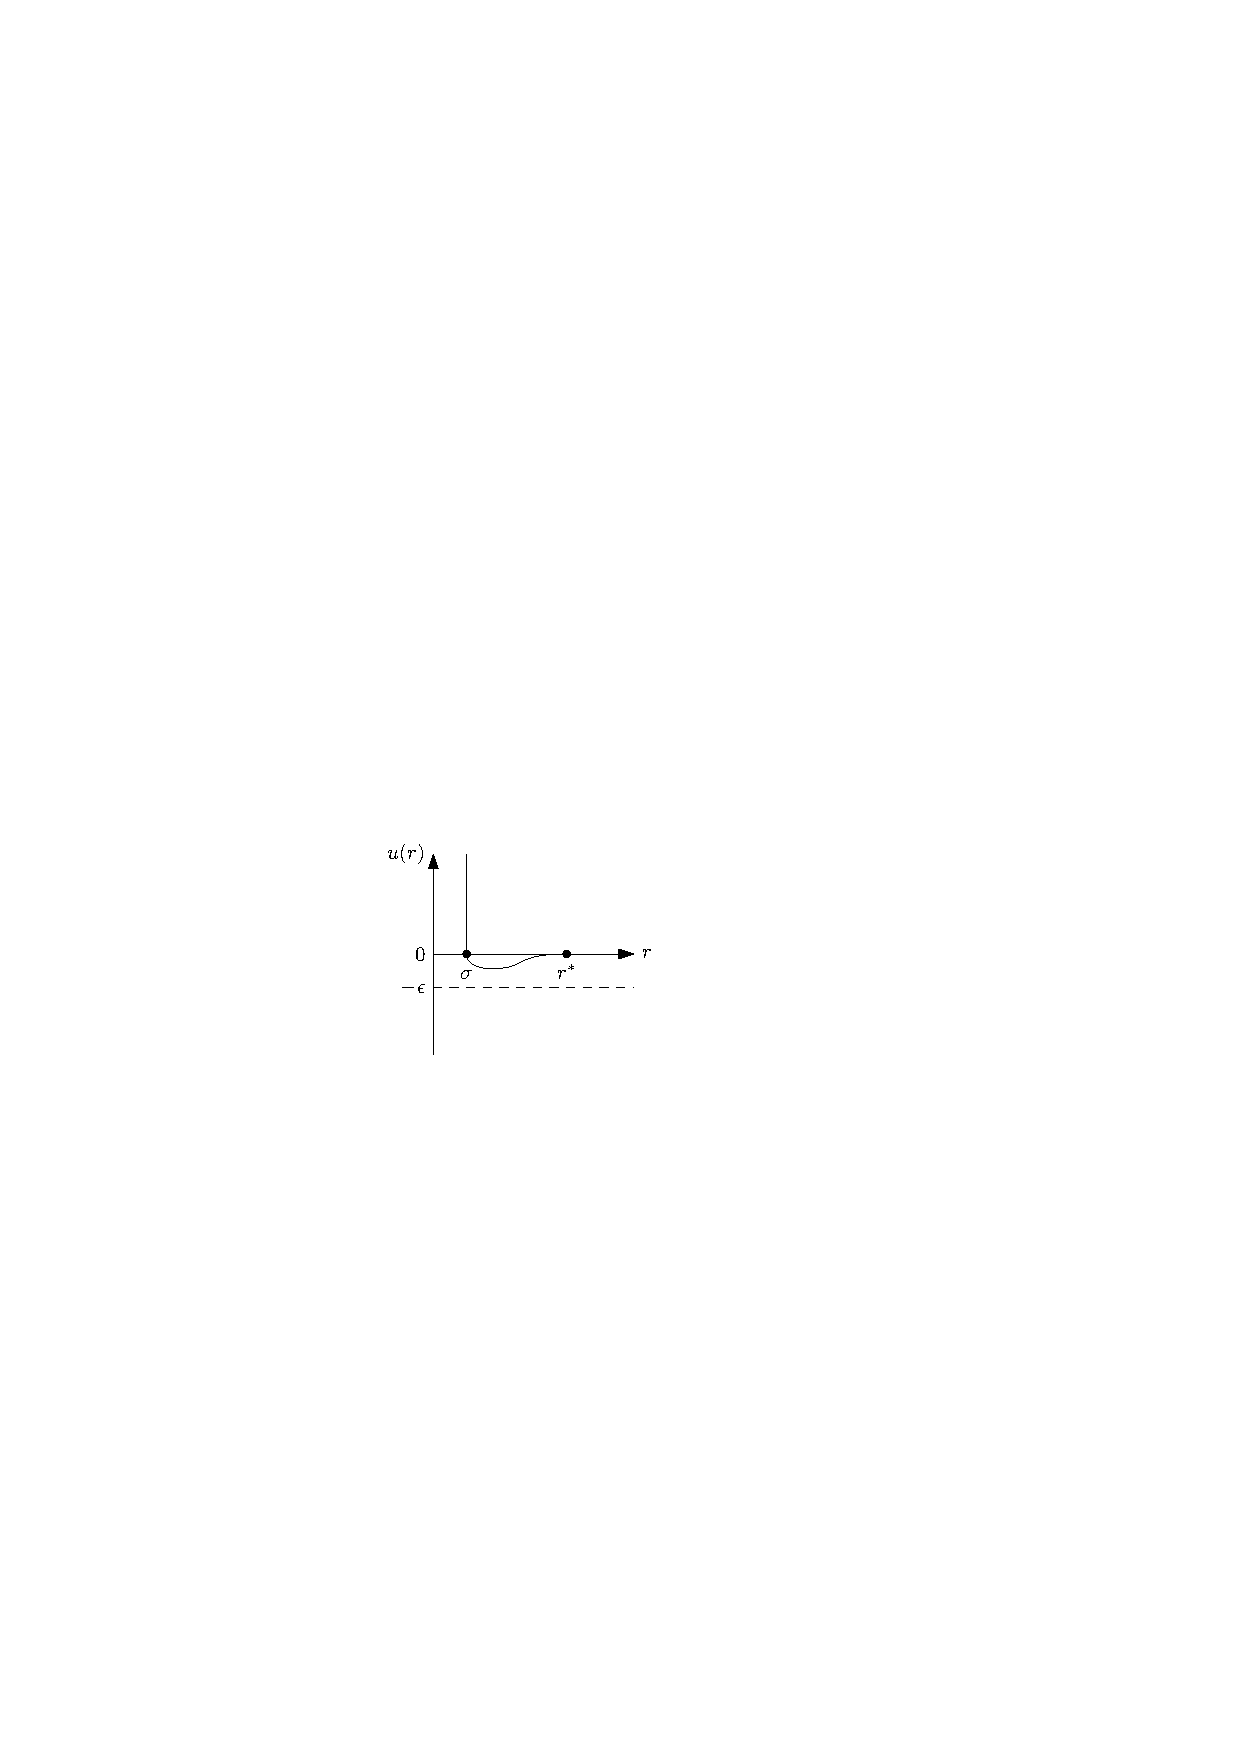
\includegraphics[scale=1]{figures/the interparticle potential.pdf}
		\caption{the interparticle potential.}
	\end{figure}
	
	\item 
\end{itemize}
